\documentclass[a4paper]{article}

\usepackage{pgfplots}

\usepgfplotslibrary{patchplots}

\begin{document}
\begin{tikzpicture}
%\tracingcommands=2\tracingmacros=2
	\begin{axis}[use fpu=false]
	\addplot[patch,domain=-1:1,patch type=cubic spline,patch type sampling,samples=5] {x^3};	
	\end{axis}
\end{tikzpicture}

\message{SURF:^^J}
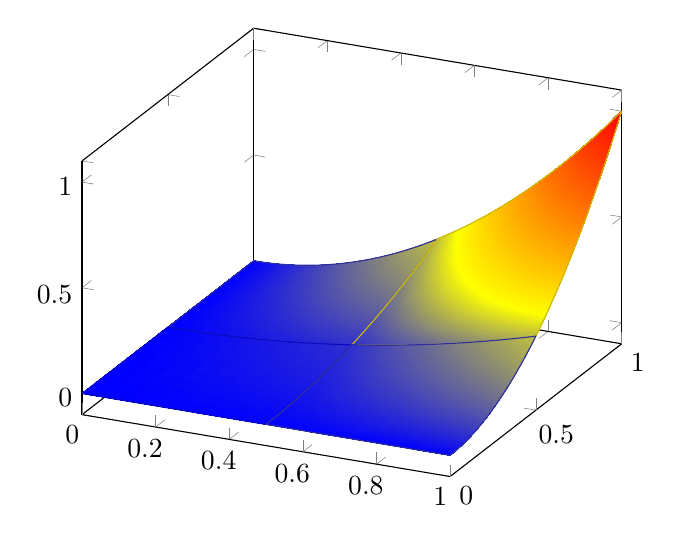
\begin{tikzpicture}
%\tracingcommands=2\tracingmacros=2
	\begin{axis}[use fpu=false]
	\addplot3[surf,shader=faceted interp,domain=0:1,patch type=biquadratic,patch type sampling,samples=3] {x^2*y^2};	
	\end{axis}
\end{tikzpicture}

\def\pgfplotspatchready{READY.}%

\foreach \x in {line,triangle,rectangle,quadratic spline,cubic spline,bilinear,triangle quadr} {
	\noindent Patch class \x:\par
	\pgfplotspatchclass{\x}{sample in unit cube}{
		Point: (\pgfplotspatchclassx,\pgfplotspatchclassy).
	}

}

\end{document}

